

\begin{frame}
\section{Pairwise clustering}

\textbf{Recall} that K-means clusters points based on their proximity to some prototype.\\

\notesonly{
Another approach to describing a similar ``structure'' in the data
can be based on the following:}
\slidesonly{
\begin{figure}[h!]
  \centering
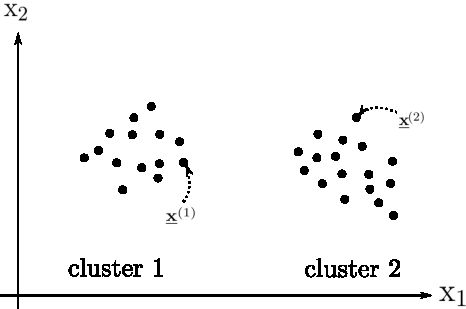
\includegraphics[height=3cm]{img/clustering} 
\end{figure}
But also:\\
}
Points that are ``close'' to one another have more in common than points that are far away from one another. 
\notesonly{
We clusters points based on their \emph{proximity to one another}. 
A point that is further away from this collection is grouped with other points that are closer to it. Pairwise clustering is about grouping points based on their pairwise relations. \
}
We will first discuss clustering based on \emph{pairwise distances} and then extend this to \emph{soft clustering}.

\end{frame}

